\documentclass{article}

\usepackage[dblblindworkshop]{neurips_2026}
\workshoptitle{Can We Trust the Judge? Reliability and Validity of LLM Evaluators
               (JUDGe), NeurIPS 2026}

\usepackage[utf8]{inputenc}
\usepackage[T1]{fontenc}
\usepackage{hyperref}
\usepackage{url}
\usepackage{booktabs}
\usepackage{amsmath}
\usepackage{amsfonts}
\usepackage{nicefrac}
\usepackage{microtype}
\usepackage{xcolor}
\usepackage{graphicx}
\usepackage{placeins}
\renewcommand{\arraystretch}{0.94}
\setlength{\abovecaptionskip}{4pt}
\setlength{\belowcaptionskip}{2pt}
\setlength{\textfloatsep}{8pt plus 2pt minus 2pt}
\setlength{\intextsep}{8pt plus 2pt minus 2pt}

\title{An LLM Judge Loses Reliability on Problems in Its Training Corpus,
       but Only When the Reference Answer Is Withheld}

\author{%
  Anonymous Author(s) \\
  Affiliation \\
  Address \\
  \texttt{email} \\
}

\begin{document}

\maketitle

\begin{abstract}
Automated evaluators are trained artifacts, so a verdict on a benchmark item may depend on
whether the evaluator itself read that item during training, yet the corpora of models
normally deployed as judges are closed and the question is usually left open. Instella
publishes its complete pretraining mixture, and its stage two component derives from the
GSM8K training split and not the test split, so membership is fixed by exact thirteen gram
containment instead of estimated: the adopted threshold flags none of 1000 known negative
test items, and the looser any match rule of Brown et al.\ flags 3, a false positive rate
of 0.3 percent. Difficulty matched arms of 250 seen and 250 unseen problems expand into
2017 candidate solutions produced by four Instella checkpoints, and three judges spanning
a capability range, Instella 3B Instruct, Qwen2.5 7B Instruct and Qwen2.5 14B Instruct,
return 48{,}408 verdicts at temperature zero under two prompts that differ only in whether
the gold answer is supplied. Chance corrected agreement is shown to be the wrong statistic
here and is reported as a cautionary result: Cohen's kappa manufactures a seen minus unseen
gap of $-0.292$ $[-0.356, -0.228]$ purely from a base rate difference of 77 against 53
percent, a textbook instance of the Feinstein and Cicchetti paradox, while balanced
accuracy on the identical verdicts puts the same cell at $+0.054$. Under balanced accuracy
a dissociation appears. Supplying the reference answer drives the membership gap toward
zero as judges improve, running $-0.054$, $-0.036$ and $-0.023$, the last spanning zero,
and toward zero more sharply still on a second generator at $-0.122$, $-0.002$ and
$+0.008$. Withholding it removes the convergence entirely, at $-0.081$, $-0.200$ and
$-0.184$, with the effect emerging exactly where a judge first becomes competent, since
control condition balanced accuracy climbs from 0.514 to 0.937 to 0.946 across the ladder.
Scale does not repair the reference free gap, which rules out a weak judge artifact.
Abstention stays between 0.0 and 2.6 percent throughout, so selective non response does not
generate the pattern. All intervals are cluster bootstraps over parent problems against a
measured intraclass correlation of 0.48, since resampling rows would contract them by a
design effect near 2.4. The practical consequence is narrow and testable: reference free
LLM grading, the configuration used whenever no gold answer exists, degrades on exactly the
items most likely to sit in a judge's training data, and supplying a reference restores it.
\end{abstract}

\section{Introduction}

Using a language model to grade another model's output rests on an assumption that is
seldom examined, that the evaluator's reliability does not depend on the material being
evaluated. If a judge has memorized a benchmark problem, its verdict on a candidate
solution to that problem may reflect what it remembers instead of what it was shown. The
verdict is then a measurement whose calibration varies with the thing being measured, which
is the property an instrument is supposed not to have.

Testing the assumption needs the judge's training corpus. For the closed weight models
usually deployed as judges that is unavailable, so existing audits study properties
observable from the outside. Zheng et al.~\citep{zheng2023judging} establish the paradigm
and document position bias, verbosity bias and self preference, and report that strong
judges agree with human preference above 80 percent of the time. None of that work can
condition on membership, because membership is not knowable for the judges in question.

Instella~\citep{instella2025} makes it knowable for one judge and one corpus. AMD publishes
the full pretraining mixture, and the stage two synthetic mathematics corpus derives from
the GSM8K training split~\citep{cobbe2021gsm8k} and not from the test split. Membership of
a problem in that corpus follows from exact thirteen gram
containment~\citep{brown2020fewshot}. Since the corpus is generated only from train, every
test item is a known negative, which converts detector error from an assumption into a
measured quantity.

That gives an item partition with verified provenance, and the study puts the same items to
three judges under two prompts differing in one respect, whether the gold answer for the
graded variant appears. The reference based condition reduces grading to comparison, so a
remembered answer buys the judge nothing. The reference free condition requires assessing
the presented reasoning, which is where recall could substitute for verification. Because
both conditions run over identical items and identical candidate solutions, the contrast
between them is internal to each judge and does not depend on what the arm label means for
that judge's own corpus, a point Section~\ref{sec:limits} returns to.

Three contributions follow. First, judge reliability measured against membership fixed by
containment rather than inferred, over 48{,}408 verdicts. Second, a dissociation in which
supplying a reference answer removes the membership gap while withholding it does not, with
the gap appearing precisely where judges become competent. Third, a documented case of the
kappa paradox producing a large and interval excluding effect on data where the effect is
absent, which is worth reporting because chance corrected agreement remains a common choice
for exactly this measurement.

\section{Design}

\paragraph{Verified arms.}
Item text is lowercased, reduced to alphanumeric tokens, and cut into every window of 13
consecutive tokens. Containment is the fraction of an item's windows appearing in the
corpus. Because the corpus derives only from GSM8K train, the test split calibrates the
rule: the any match convention of Brown et al.~\citep{brown2020fewshot} flags 3 of 1000
known negatives, and the threshold adopted here flags none of them. Identifiers are
namespaced by split, without which train and test items collide and containment exceeds
unity. From the eligible pools, 250 seen and 250 unseen parent problems are drawn matched on
reasoning step count, so arm composition cannot stand in for a membership effect.

\paragraph{Candidate solutions.}
Each parent expands into one original and four variants, two answer preserving and two
answer changing, giving 2017 rows. Four Instella checkpoints generate candidate solutions
under pinned decoding, and exact match against ground truth supplies the label each judge is
scored against. Two thirds of graded rows are variants, and the answer changing variants
carry different correct answers from their originals, which matters for the mechanism in
Section~\ref{sec:mech}.

\paragraph{Judges and conditions.}
Three judges span a deliberate capability range: Instella 3B Instruct, Qwen2.5 7B Instruct
and Qwen2.5 14B Instruct. Each emits one word, correct or incorrect, at temperature zero
under a 24 token budget. The two conditions differ in one element of the prompt. Reference
based grading supplies the gold answer for the variant at hand and is the control, since
recall of a remembered solution cannot help once the solution is given. Reference free
grading withholds it.

\paragraph{Metric and inference.}
Balanced accuracy, the unweighted mean of sensitivity and specificity, is used throughout.
Both components condition on the true class, so neither moves with the base rate, and their
mean stays comparable across arms whose ground truth composition differs. Chance is 0.5.
Section~\ref{sec:kappa} shows why the obvious alternative fails here. Intervals are
bootstraps over parent problems rather than rows, because the five rows of one problem are
not five independent observations; the measured intraclass correlation is approximately
0.48, and resampling rows would contract intervals by a design effect near 2.4.

\section{Results}

\subsection{Chance corrected agreement is the wrong statistic here}
\label{sec:kappa}

Judge accuracy was first measured as Cohen's kappa against exact match ground truth, and the
result looked conclusive. Grading stage two outputs, the seen minus unseen difference came
to $-0.292$ on an interval of $[-0.356, -0.228]$, and grading instruct outputs $-0.168$ on
$[-0.228, -0.113]$. Both exclude zero by a wide margin and both point the same way.

The effect is an artifact of the marginals. Kappa depends on the marginal distributions as
well as on agreement, and the arms have very different ground truth base rates: the instruct
generator is correct on 77 percent of seen rows against 53 percent of unseen. An arm sitting
near one half has far more chance corrected headroom than a skewed arm, so the skew alone
produces a gap. Feinstein and Cicchetti~\citep{feinstein1990kappa} describe this as the first
of two kappa paradoxes, in which high raw agreement is driven down by marginal imbalance.
Figure~\ref{fig:kappa} puts both statistics on the same verdicts. Kappa separates the arms by
0.292; balanced accuracy separates them by 0.054 in the opposite direction.

\begin{figure}[t]
\centering
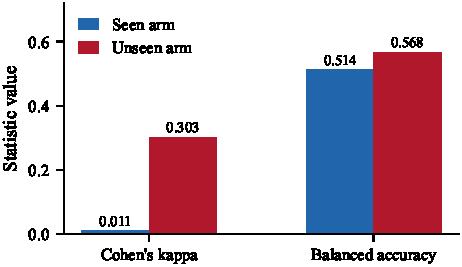
\includegraphics[width=0.52\linewidth]{judge_fig3_kappa.pdf}
\caption{Two statistics computed on one set of verdicts, Instella 3B Instruct grading stage
two outputs in the reference free condition. Cohen's kappa reports a large seen minus unseen
gap that reflects a ground truth base rate difference of 77 against 53 percent between the
arms. Balanced accuracy, which conditions on the true class, does not.}
\label{fig:kappa}
\end{figure}

Reporting this is not incidental. Chance corrected agreement is a standard choice for judge
reliability, and on a design where the arms differ in difficulty it will manufacture a
membership effect from nothing.

\subsection{The dissociation}

Table~\ref{tab:diss} and Figure~\ref{fig:diss} give the membership gap in balanced accuracy
under both conditions. Supplying the reference answer produces the behaviour a control
should show: as judges improve the gap contracts toward zero, from $-0.054$ to $-0.036$ to
$-0.023$, with the strongest judge spanning zero. On candidate solutions from the stage two
generator the convergence is sharper, running $-0.122$, then $-0.002$, then $+0.008$.

\begin{table}[t]
\centering
\caption{Balanced accuracy, seen minus unseen, grading instruct outputs. Intervals are 95
percent bootstraps over parent problems, 4000 draws. An asterisk marks an interval excluding
zero.}
\label{tab:diss}
\small
\begin{tabular}{lcc}
\toprule
Judge & Reference given (control) & Reference withheld \\
\midrule
Instella 3B Instruct  & $-0.054$ [$-0.083$, $-0.026$]$^{*}$ & $-0.081$ [$-0.109$, $-0.054$]$^{*}$ \\
Qwen2.5 7B Instruct   & $-0.036$ [$-0.068$, $-0.008$]$^{*}$ & $\mathbf{-0.200}$ [$-0.248$, $-0.149$]$^{*}$ \\
Qwen2.5 14B Instruct  & $-0.023$ [$-0.057$, $+0.006$]       & $\mathbf{-0.184}$ [$-0.231$, $-0.133$]$^{*}$ \\
\bottomrule
\end{tabular}
\end{table}

Withholding the reference removes the convergence. The gap grows once a judge is strong
enough to show it and then holds, at $-0.081$, $-0.200$ and $-0.184$. A defect of small
models would shrink as capability rises. This does the opposite between the first and second
judge and then flattens.

\begin{figure}[t]
\centering
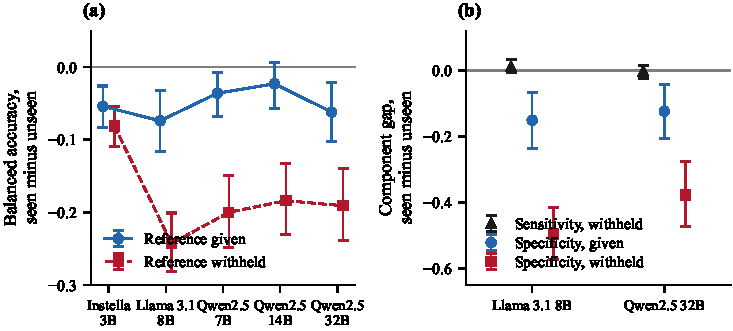
\includegraphics[width=0.48\linewidth]{judge_fig1_dissociation.pdf}
\hfill
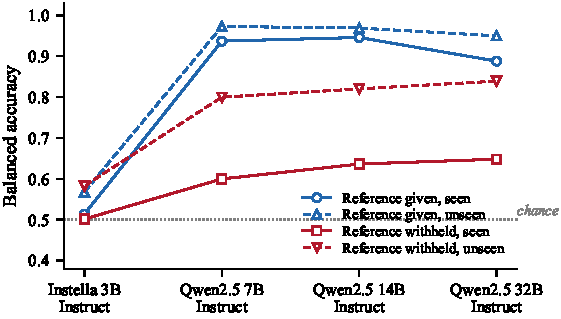
\includegraphics[width=0.48\linewidth]{judge_fig2_ladder.pdf}
\caption{Left: membership gap in balanced accuracy across the judge ladder under both
conditions, grading instruct outputs. Right: absolute balanced accuracy for all four cells
of the design. The control condition confirms the two larger judges are competent
instruments, reaching 0.94 to 0.97, so the reference free result is not read off a judge
that cannot grade.}
\label{fig:diss}
\end{figure}

\subsection{Capability is demonstrated rather than assumed}

A null or an effect from an incompetent judge says nothing, so absolute performance is
reported alongside the gaps. Table~\ref{tab:ladder} gives every cell. Given the reference
answer, the 7 and 14 billion parameter judges reach 0.937 to 0.973, which is the regime in
which their reference free numbers become interpretable. The 3 billion parameter judge sits
within 0.04 of chance on the seen arm in every configuration, including when handed the
answer, so its rows describe a noise floor and the substantive claims rest on the larger two.

\begin{table}[t]
\centering
\caption{Absolute balanced accuracy per cell, grading instruct outputs. Chance is 0.500.}
\label{tab:ladder}
\small
\begin{tabular}{lcccc}
\toprule
& \multicolumn{2}{c}{Reference given} & \multicolumn{2}{c}{Reference withheld} \\
\cmidrule(lr){2-3}\cmidrule(lr){4-5}
Judge & Seen & Unseen & Seen & Unseen \\
\midrule
Instella 3B Instruct  & 0.514 & 0.568 & 0.502 & 0.583 \\
Qwen2.5 7B Instruct   & 0.937 & 0.973 & 0.600 & 0.800 \\
Qwen2.5 14B Instruct  & 0.946 & 0.969 & 0.636 & 0.820 \\
\bottomrule
\end{tabular}
\end{table}

Three readings follow from the table taken together with Table~\ref{tab:diss}. Capability is
real, so conclusions about the instrument come from instruments that work. The control
behaves as a control, since supplying the correct answer for the specific variant removes
the gap, which is what a recall account predicts and a pure difficulty account does not.
And the reference free gap neither converges nor responds to scale.

\subsection{Abstention and what would falsify the account}

A judge that declines to answer more often on one arm could produce the whole pattern with no
change in grading quality at all, since abstentions removed from the denominator reshape both
sensitivity and specificity. Abstention stays between 0.0 and 2.6 percent across every judge,
condition and arm, which is too small and too evenly spread to carry a gap of 0.200.

Three outcomes would have contradicted the account, and none occurred. Had the reference free
gap shrunk with capability in the way the control gap does, the effect would be a defect of
weak judges; instead it grows from the first judge to the second and then holds. Had the
control gap failed to converge, the arms would differ in some way that persists even when the
answer is supplied, pointing at difficulty rather than at recall; instead the strongest judge's
control interval spans zero. And had the two larger judges failed to clear chance in the
control condition, no reading of their reference free numbers would be available at all;
instead they reach 0.937 and 0.946 on the seen arm.

\section{Implications for evaluator construct validity}

An evaluator is valid for a construct when its verdicts track that construct and nothing else.
The results here describe a specific and narrow failure of that condition. Under reference free
grading the measured quantity is not solely the quality of the reasoning presented, because it
also varies with whether the graded problem is one the evaluator is likely to have read. The
variation is not small: 0.200 in balanced accuracy on the 7 billion parameter judge, against a
control gap of 0.036 on the identical items and the identical candidate solutions.

Two practical consequences follow. Reference free grading is the configuration used exactly
where a gold answer does not exist, which includes open ended generation, proof sketches, and
any setting where the task is to assess a chain of reasoning on its own terms, so the failure
falls on the applications that most need a trustworthy judge. And a benchmark assembled from
public sources is the case where the affected items are most concentrated, since public
availability is what puts an item in a training corpus in the first place. Supplying a
reference answer, where one exists, removes the effect in these data, which makes it a
mitigation rather than merely a diagnosis.

\section{Mechanism}
\label{sec:mech}

The pattern fits substitution of recall for verification. Asked to grade a problem present
in its training data without being told the answer, a judge appears to check the candidate
solution against the answer it remembers instead of against the reasoning in front of it.
Two thirds of graded rows are variants, and the answer changing variants have different
correct answers from their originals, so a remembered answer marks correct solutions wrong.
Supplying the reference for the variant at hand removes any need to recall, and the gap goes
with it.

The account is inferential. Establishing it directly would require attributing a verdict to
a specific memorized document, which the present data cannot do.

\section{Limitations}
\label{sec:limits}

\paragraph{Membership is verified for one judge, and it is not the judge carrying the
result.} Containment is measured against the Instella corpus. The Instella judge therefore
has verified membership but sits at chance. The Qwen judges show the effect, and their
corpora are unknown, so for them the partition is GSM8K train against test rather than
verified seen against unseen. This asymmetry is real and is the main reason the primary
claim is stated as a within judge contrast between two conditions over identical items and
identical candidate solutions, which holds whatever the arm label means for a given judge.
What the Qwen results establish is that a competent judge grades this partition differently
depending on whether a reference is supplied. Closing the gap between that and a membership
claim requires a second open corpus model of comparable capability.

\paragraph{One family supplies the candidate solutions.} Every graded output comes from an
Instella checkpoint. Whether the dissociation reproduces on solutions from other generators
is untested.

\paragraph{One checkpoint is unexplained.} The effect concentrates on stage two and instruct
outputs. Stage one outputs are wrong nearly everywhere and are trivially gradeable in either
condition, which accounts for that null. The supervised fine tuned checkpoint shows no gap in
either condition despite output quality comparable to instruct, and the present data do not
explain why.

\paragraph{Mechanism is inferred, and one prompt template is tested.} No attribution evidence
links a verdict to a training document, and robustness of the dissociation to prompt phrasing
is untested.

\section{Conclusion}

Measured against membership fixed by containment rather than estimated, an LLM judge shows no
loss of reliability on problems from its training corpus when the reference answer is
supplied, and a substantial one when it is withheld. The gap under reference free grading
runs to 0.200 in balanced accuracy and does not close with scale, while the same judges in
the control condition converge toward zero as they improve. Chance corrected agreement
inverts this picture on identical verdicts and should not be used where the arms differ in
base rate. The operational reading is specific: reference free grading is the configuration
deployed whenever no gold answer exists, and it is the configuration in which the items most
likely to be in a judge's training data are graded least reliably.

\bibliographystyle{plainnat}
\bibliography{judge}

\newpage
\appendix

\section{Related work in full}

Zheng et al.~\citep{zheng2023judging} introduce the LLM as judge paradigm at scale and
document position bias, verbosity bias and self preference, reporting agreement with human
preference above 80 percent for strong judges. Their audits characterize the judge and the
prompt; membership of the graded item in the judge's corpus is outside reach for the closed
models they study, which is the gap the present design addresses for one open family.

On the detection side, containment based overlap rules originate with
Brown et al.~\citep{brown2020fewshot}, and membership inference from model confidence is
developed by Carlini et al.~\citep{carlini2023quantifying} and
Shi et al.~\citep{shi2024detecting}. Yang et al.~\citep{yang2023rephrased} show that
rephrasing defeats overlap based detection outright, which is why a study that needs a
trustworthy treatment label cannot rely on an estimated one.

Two lines of work establish the value of released intermediate checkpoints.
Biderman et al.~\citep{biderman2023pythia} release the Pythia suite specifically to make
training dynamics analyzable, and Biderman et al.~\citep{biderman2023emergent} use such
checkpoints to study when memorization emerges during training. The present work applies the
same logic to an evaluator rather than to a generator.

\section{Containment method and calibration}

Item text is normalized to lowercase alphanumeric tokens and decomposed into every window of
13 consecutive tokens. Containment against a corpus is the fraction of an item's windows
found in it, computed in one streaming pass with an inverted index from window to source
item, so cost is linear in corpus size and independent of how many item sets are indexed
together. Because the corpus is generated only from the GSM8K training split, every test item
is a verified negative: the any match rule flags 3 of 1000, a rate of 0.3 percent, and the
adopted threshold flags none.

Identifier namespacing is load bearing. GSM8K train and test share an index scheme, so
loading both without namespacing collides items and produces containment values above unity,
which is impossible for a fraction. Anyone reproducing this design will meet the same trap.

\section{Reproducibility controls}

Several controls are load bearing rather than incidental. The transformers version is pinned
exactly, since a version range places different checkpoints on different minor versions and
that difference enters the estimate as though it were a model difference. Batch size is fixed
across all generation, because greedy decoding in reduced precision is sensitive to padding
and a batch size change alters tie breaking. Variants are seeded per pair of item and
perturbation type, so variant text is stable regardless of call order and generations stay
valid when the item set changes. Every generation batch is flushed to disk and resume is
keyed on item identifier, so an interrupted run continues instead of restarting.

All generation records, containment values, judge verdicts and analysis code are released for
audit at a public repository and dataset mirror, both anonymized for review. Random seeds are
fixed across arm selection, variant construction and every bootstrap. An assistant helped
implement generation, containment and analysis code under the direction of the authors, who
verified every reported number against the underlying verdict files; the assistant did not
design the conditions or choose which results to report.

\end{document}
